\documentclass[11pt]{article}

\usepackage[width=7.0in, height=9.0in, top=1.0in, papersize={8.5in,11in}]{geometry}
\usepackage[pdftex]{graphicx}
%\usepackage{datetime}
\usepackage{anyfontsize}
\usepackage{t1enc}
\usepackage{verbatim}
\usepackage{algorithm}
\usepackage{algorithmic}
\usepackage{framed}
\usepackage{pdfpages}
\usepackage{listings}
\lstset{language=C}

\lstset{language=python,frame=ltrb,framesep=5pt,basicstyle=\normalsize,
 keywordstyle=\ttfamily\color{DarkRed},
%morecomment=[n][\textbf]{In\ [}{]\:},
%morecomment=[n][\textbf]{Out\ [}{]\:},
morecomment=[s][\color{blue}]{In\ [}{]\:},
morecomment=[s][\color{red}]{Out[}{]\:},
identifierstyle=\ttfamily\color{DarkBlue}\bfseries,
commentstyle=\color{DarkGreen},
stringstyle=\ttfamily,
showstringspaces=false,tabsize = 3}

  
\lstdefinelanguage{shell} {
commentstyle = \color{black},
keywordstyle = \color{black},
stringstyle = \color{black},
identifierstyle = \color{black},
morecomment=[s][\color{blue}]{In\ [}{]\:},
morecomment=[s][\color{red}]{Out[}{]\:},
 }

\pagestyle{empty}

\usepackage{helvet}
\usepackage{titlesec}
\usepackage{graphicx}
\usepackage{wrapfig}
\usepackage[font=scriptsize]{caption}


\renewcommand{\familydefault}{\sfdefault}


\titleformat{\section}
  {\normalfont\Large\bfseries}{\thesection}{1em}{}[{\titlerule[0.8pt]}]
  
\title{\textbf{Prototype Sprint \#1}}
\date{}

\begin{document}


\maketitle

\section*{Project Overview}

The capability of UAVs to rapidly search a large area, especially an area that is difficult to traverse by foot or vehicle, would be invaluable to operations such as search \& rescue. However, small UAVs have a very limited flight time.\\

\noindent A system incorporating a UVG equipped with a landing pad that also serves as a charging station would allow the UAV to be delivered to areas of limited access. The UAV could then, being provided with waypoints by the user, autonomously take-off, and navigate through the waypoints. After moving through the waypoints, or when the UAV requires recharging, the UAV will return to the UVG and safely land in such a way that the charging unit can connect to the UAV.\\

\noindent Team Expeditus aims to specifically create and deliver software that allows a UAV to autonomously take-off, navigate to way-points designated by the user, and return to the landing pad in manner that allows for charging and redeployment. 

\section*{Goals}
\begin{itemize}
\item Autonomous Take-off
\begin{itemize}
\item Reaching a specific height before navigation
\item Provided no obstacles in reaching operating height
\end{itemize}

\item Autonomous Navigation of Waypoints
\begin{itemize}
\item Provided an obstacle free operation space
\end{itemize}

\item Autonomous Landing of UAV that is:
\begin{itemize}
\item Accurate within +/- .1 meters
\item Oriented correctly
\end{itemize}
\end{itemize}


\section*{Approach}

\textbf{Phase I}\\
This first phase requires the testing of hardware and ensuring the quadrotor is properly configured and is capable of stable and controllable flight. This will mean many iterations of manual flight. Take-off and way-point navigation is solved by the use of MavLink. Testing of these capabilities will first be tested through the use of Mission Planner or APM Planner, which provides a handy interface for setting up take-off and way point navigation. The last goal of this phase will be a simulation environment to simulate landing algorithms.\\

\noindent \textbf{Objectives}
\begin{enumerate}
	\item Test of Manual Flight
	\item Test of Mavlink Autonomous Control
	\item Setting up Simulation Evironment for Quadrotor
\end{enumerate}

\noindent \textbf{Phase II}

\begin{wrapfigure}{r}{0.4\textwidth}
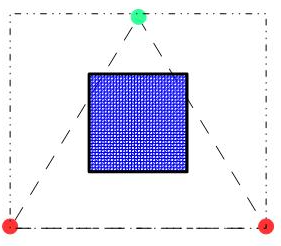
\includegraphics[width=0.4\textwidth]{landing_pad}
\caption{Landing Pad Light \& QR Code Layout}
\label{fig:landing_pad}
\end{wrapfigure}

\noindent Computer vision has been determined to hold the most promise to solve the landing goal. Autonomous landing provided by the GPS (detailed in the hardware section below) provides an accuracy of nav-point navigation, given optimal conditions, to within $+/-$10 meters. This is obviously unsatisfactory to use for purposes of landing on a small platform, but it should bring us within a distance of our goal to detect the landing platform from our downward facing camera. \\

\noindent \textit{Lights}: Colored lights arranged in either a rectangle or triangle with different colors on selected lights(figure~\ref{fig:landing_pad}) to provide orientation information for the UAV. The warping and scale of the shape would provide the orientation by the operation needed to unwarp the shape, and the scale would provide distance information. The UAV will use the lights to provide information to the flight controller to manuever above the landing pad at a certain height, and with a specific orientation before switching state to use the QR code.\\

\noindent \textit{QR Code}: Similar to the lights, warping and scale will provide the UAV with information regarding the orientation and distance between the UAV and the QR code. The QR code will be centered on the landing pad(figure~\ref{fig:landing_pad}).The UAV will be generally centered above the landing pad and at a much closer height, and so this state will be the last fine maneuvers of the UAV to land accurately and with the correct orientation.\\

\noindent ROS will be used as the glue to allow the communications(figure~\ref{fig:ROS}) needed between camera, flight controller, and Odroid. Although ROS is not a real-time operating system, it has near real-time capability provided through use of ROS communication tools such as actions, which can provide needed interrupts to activities, and switch state. As the UAV nears the platform, the state will change with the initial image acquisition of the landing platform. This state change will initiate controls to be fed from the software on the Odroid to the flight controller to bring the UAV onto the landing pad with accuracy and correct orientation. 
\begin{enumerate}
\item Test Autonomous Landing Capability in Simulation
\item Implement Autonomous Landing Capability
\item Test Autonomous Landing Capability
\item Tie Capabilities together
\item Final Testing of UAV with Landing Pad
\end{enumerate}

\begin{figure}[h]
\centering
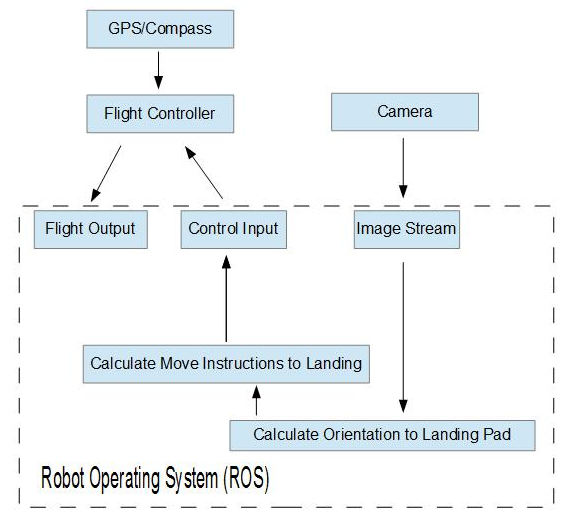
\includegraphics[width=0.5\textwidth]{UAV_Control_1}
\caption{General ROS \& Flight Control Setup}
\label{fig:ROS}
\end{figure}

\section*{Components}
\begin{figure}[h]
\centering
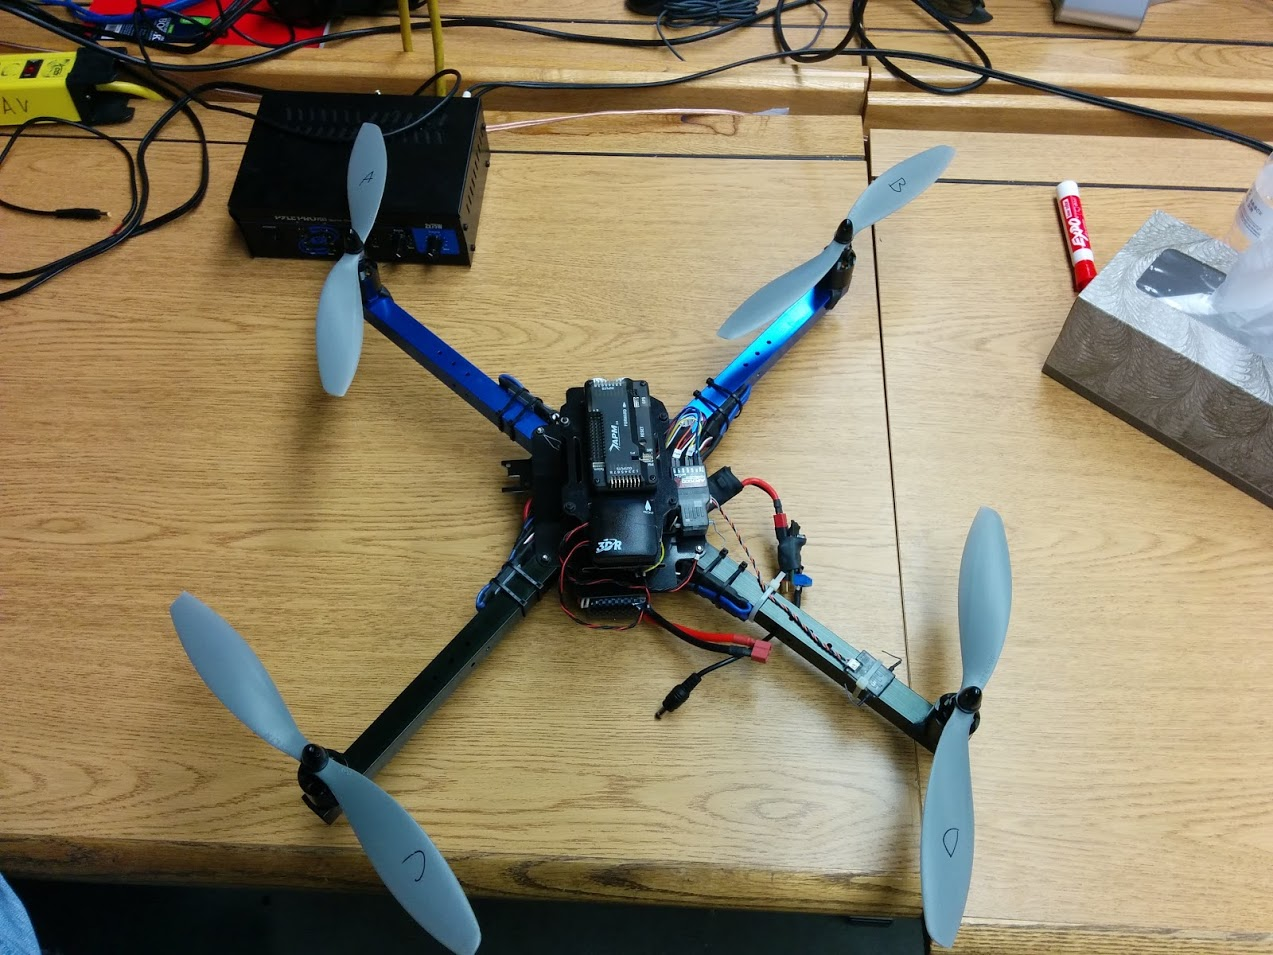
\includegraphics[width=0.5\textwidth]{UAV}
\caption{Current UAV Build}
\label{fig:UAV}
\end{figure}


\noindent \textbf{UAV Hardware}\\
The hardware platform is a quadrotor that had been assembled from a previous iteration of the project(figure~\ref{fig:UAV}). To achieve our goals, replacement parts will need to be ordered, as well as some additional equipment to allow the Odroid to coordinate specific landing commands given evaluation of images it receives(figure~\ref{fig:UAV_2}). The platform consists of:

\begin{itemize}
\item \textit{APM 2.6+ Assembled}: This serves as the flight controller for the quadrotor. It includes a 3-axis gyro, accelometer, and barometer. It is protected within an enclosure.
\item \textit{3DR uBlox GPS with Compass Kit}: GPS and Compass unit with enclosure, external to flight controller to be located on the quadrotor where magnetic interference is least. 
\item \textit{DIY Quad Kit}: Kit consisting of body and other components such as:
\begin{itemize}
\item Landing Struts(4)
\item 850kV motors(4)
\item Power Distribution Board
\item Electronic Speed Controllers(4)
\item Propellers(4)
\item Power Module \& Adapter
\item Radio module
\item Transmitter
\end{itemize}
\end{itemize}

\begin{figure}[h]
\centering
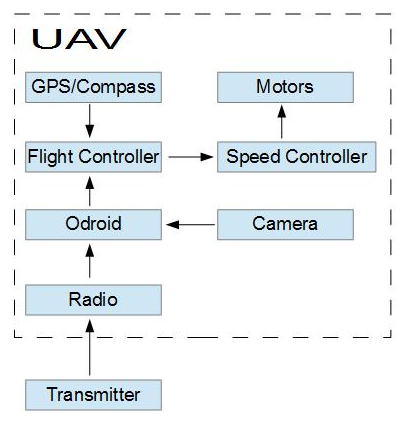
\includegraphics[width=0.5\textwidth]{UAV_Control_2}
\caption{General Hardware Configurations}
\label{fig:UAV_2}
\end{figure}

\noindent \textbf{Additional Hardware}
\begin{itemize}
\item \textit{USB Camera(2)}: To be used in conjunction with Odroid to provide image stream.
\item \textit{Odroid XU4}: To be used to process images and provide instructions to the flight controller during the autonomous landing phase.
\end{itemize}

\noindent \textbf{UAV Software}\\
Team Expeditus will take advantage of developed software that interfaces and controls the quadrotor. As stated previously, this will provide the autonomous take-off and waypoint navigation. To achieve autonomous landing, the flight controller API will be used as a node within a ROS system. 
\begin{itemize}
\item \textit{Mission Planner (Windows)}: To be used during testing autonomous take-off flight and way-point navigation.
\item \textit{APM Planner( Windows/Linux)}:  Alternative to Mission Planner, has Linux support.
\item \textit{MavLink}: API to receive output from the flight controller, as well as providing instructions to the flight controller.
\end{itemize}

\noindent \textbf{Additional Software}
\begin{itemize}
\item \textit{OpenCV}: Provides a open-source library with image processing and computer vision capabilities.
\item \textit{ROS (Robot Operating System)}: An open-source pseudo-operating system employing network communications to link together component functionality to allow fast prototyping and implementation of real robots.
\item \textit{MavROS}: A ROS-ified version of MavLink. It functions as a node within the ROS framework.
\item \textit{Gazebo}: A simulation environment that can be linked with ROS.
\end{itemize}

\section*{Development Environment}
\textbf{Hardware:}
\begin{itemize}
\item \textit{Assembly \& Repair}: The team has access to the Robotics Lab within the McLaury Bldg on the SDSMT campus. This lab is equipped with all necessary tools for removing, replacing, or otherwise altering the hardware configuration.
\item \textit{Flight Training}: The SDSMT UAV Team has provided orientation and access to a UAV flight simulator, so that team members are able to train on manual flight control.
\end{itemize}

\noindent \textbf{Software:}
\begin{itemize}
\item \textit{Language}: C++ will be used for the project. No other language is currently forecasted for use.
\item \textit{OS}: Development will mostly be conducted in Ubuntu 14.04 which supports the current version of ROS \& Gazebo. Current versions of Windows may be used briefly to test hardware through the use of Mission Planner.
\end{itemize}

\section*{Immediate Needs}

\textbf{Hardware:}
\begin{itemize}
\item \textit{APM 2.6+ Assembled}: Unit was unresponsive during testing.
\item \textit{3DR uBlox GPS with Compass Kit}: Unit was unresponsive during testing. Visual inspection revealed a crack across entire enclosure.
\item \textit{Odroid XU4}: Missing.
\item \textit{Landing Struts(8)}: Missing.
\item \textit{USB Cameras(2)}: Required for image capture.
\end{itemize}

\noindent \textbf{Software:}
\begin{itemize}
\item None
\end{itemize}



\end{document}